\documentclass[../main.tex]{subfiles}
%\usepackage{xr}
\usepackage{silence}
\WarningFilter{glossaries}{No \printglossary or \printglossaries found}

\begin{document}

\ifSubfilesClassLoaded{%
    \graphicspath{{figures/1-Introduction/}}%
    % \externaldocument{chapters/2-Background}%
    % \externaldocument{chapters/3-SOTA}%
    % \externaldocument{chapters/4-AttOmics}%
    % \externaldocument{chapters/5-CrossAttOmics}%
    % \externaldocument{chapters/6-Interpretability}%
    % \externaldocument{chapters/7-Conclusions}%
}{
    \graphicspath{{../figures/1-Introduction/}}%
}

\chapter{Introduction}

% \begin{chapterabstract}
%     \lipsum[1]
% \end{chapterabstract}
\minitocpage

why this thesis.
introduce precision medicine,
all the same but also all different, ex codéine, responder/non responder to some therapies.
patient oriented
access to many data, imaging, high throughput, new diagnosis -> access new info about patient but in very large quantities, high level of details, molecular process, high resolution
image well established, focus on molecular data or omics profile, unstructured data
require new tools to help improve diagnosis, new resolution also allow new way to treat patients, choose the medicine that should provide the best results.
what are those tools, IA, define IA field of IA ML
advatages/ drawbacks of ML
intorduce DL, why? benefits? requirements: large amount of data, flexible nice various type of data
motivation DL, response to drawbacks of ML approach
well estbalished in many domains
possible tasks in precision medicine: diagnosis, prognosis, treatment adequation


need of interpretability, explanation, IA Act
model intepretation?
different goals: understand model/process or find biomarkers

lead to this thesis, objectives,
benefits of DL for studying omics data, single omics
integration of omics data
can we identify biomarkers or explain the prediction
content


\section{Une première section}
\section{Deuxième section}

 %\cite{Linardatos2021_ExplainableAI}
 greihg  iopgte r\cref{fig:attomics_arch}\cref{fig:attomics_C} njjrj \cref{fig:attomics_D}, %\crefrange{fig:attomics_A}{fig:attomics_C} but %\cref{fig:attomics_A, fig:attomics_C}
 \subref{fig:attomics_A}

 Text \crefrange{sub@fig:attomics_A}{sub@fig:attomics_C}

 Let \( \mathcal{T} \) be a topological space, a basis is defined as
 \[
     \mathcal{B} = \left\{B_{\alpha} \in \mathcal{T}\, |\,  U = \bigcup B_{\alpha} \forall U \in \mathcal{T} \right\}
 \]

 Multi omics \(N\)-integration vs \(P\)-integration
 N-Integration is the framework of having multiple datasets which measure different aspects of the same samples.
 P-integration several studies of the same omic type
 \begin{figure}[htbp]
     \centering
     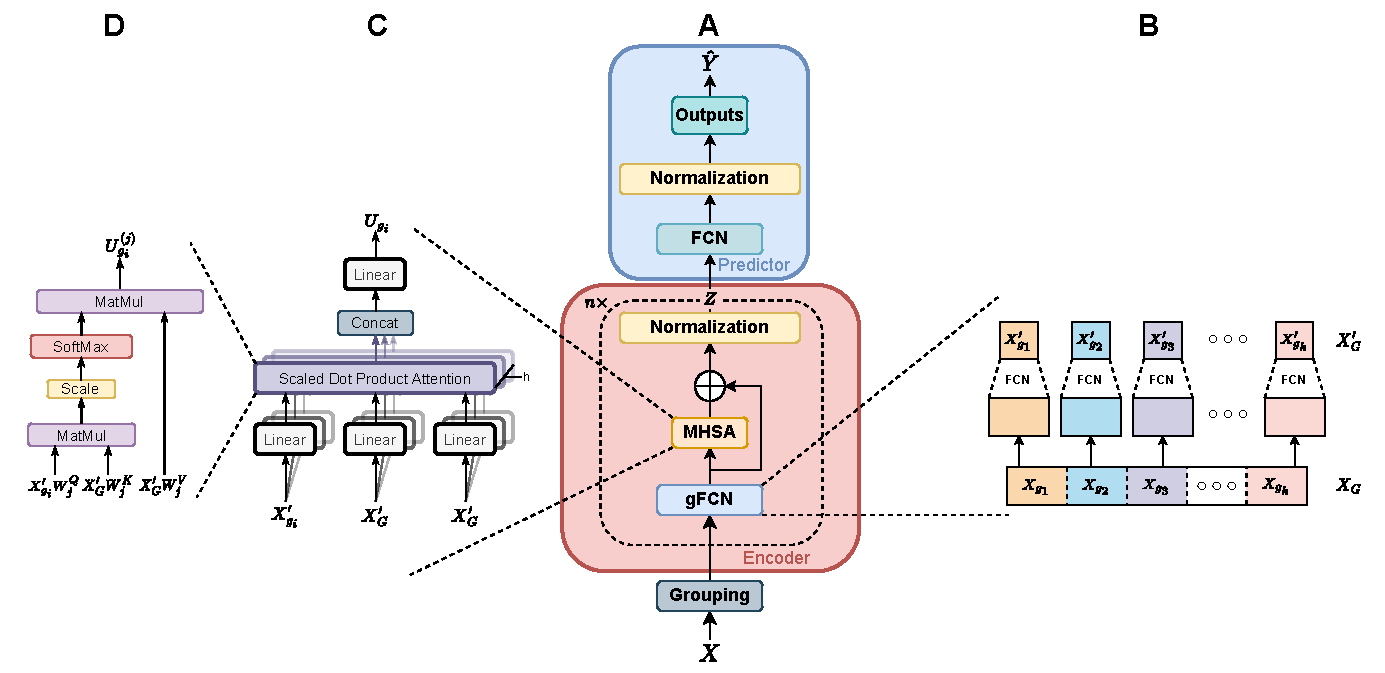
\includegraphics[width=\textwidth]{Beaude.168.fig.1.pdf}
     \caption{Cpation for this awesome figure done with pgf from matplotlib}\label{fig:enter-label2}
 \end{figure}


 \begin{table}[htbp]
     \centering
     \caption{Table caption iezofhz vroevi pero ve ervg gfre Caption}\label{tab:my_label}
     \begin{tblr}{|lccr|}
         \toprule[purple]
         Alpha   & Beta  & Gamma  & Delta \\
         \midrule[2pt]
         Epsilon & Zeta  & Eta    & Theta \\
         \hline\hline[dotted]\hline
         Iota    & Kappa & Lambda & Mu    \\
         \bottomrule
     \end{tblr}
 \end{table}

 \begin{figure}
     \centering
     \begin{tikzpicture}
         \node (in_A) at (0,0) [inner sep=1pt] {A};
         \node (in_C) [below=2cm of in_A.south, anchor=north, inner sep=1pt] {C};
         \node (in_B) [below=2cm of in_C.south, anchor=north, inner sep=1pt] {B};

         \foreach \lab in {A, B, C}
             {
                 \node (enc_\lab) [draw, thick, rounded rectangle, rounded rectangle west arc=none, right=5mm of in_\lab.east, anchor=west] {\textit{Enc}};
                 \draw[thick, -stealth] (in_\lab.east) -- (enc_\lab.west);
             }

         \path (enc_A.south) -- (enc_C.north) node[midway, draw, thick, rounded corners=5, anchor=center, xshift=2.2cm] (cross_AC) {CrossAttention};
         \path (enc_C.south) -- (enc_B.north) node[midway, draw, thick, rounded corners=5, anchor=center, xshift=2.2cm] (cross_BC) {CrossAttention};
         \path let \p1=(cross_AC.center), \p2=(cross_BC.center), \n1={veclen(\x2-\x1,\y2-\y1)} in node[below=\n1 of cross_BC.center, anchor=center, draw, thick, rounded corners=5] (cross_AB) {CrossAttention};

         \draw [-stealth, thick, rounded corners=5] (enc_C.east) -| (cross_BC.north);
         \draw [-stealth, thick, rounded corners=5] (enc_C.east) -| (cross_AC.south);
         \draw [-stealth, thick, rounded corners=5] (enc_B.east) -| (cross_BC.south);
         \draw [-stealth, thick, rounded corners=5] (enc_B.east) -| (cross_AB.north);
         \draw [-stealth, thick, rounded corners=5] (enc_A.east) -| (cross_AC.north);
         \coordinate (xx1) at (enc_A.east -| cross_AC.west);
         \path (enc_A.east) -- (xx1) coordinate [midway] (mid1);
         \path let \p1=(enc_A.east), \p2=(cross_AB.south west), \p3=(cross_AC.north), \n1={veclen(\x1-\x1,\y2-\y1)}, \n2={veclen(\x1-\x1, \y3-\y1)}, \n3={\n1 + \n2} in coordinate [below=\n3 of mid1] (mid2) coordinate [below=\n2 of cross_AB.south] (mid3);
         \draw [-stealth, thick, rounded corners=5] (enc_A.east) -- (mid1) -- (mid2) -- (mid3) -- (cross_AB.south);

         \foreach \t in {AC, BC, AB} {
                 \node (Z_\t) [inner sep=1pt, right=3mm of cross_\t.east] {\(Z_{\t}\)};
                 \draw[thick, -stealth] (cross_\t.east) -- (Z_\t.west);
                 \node at ([xshift=0.5ex, yshift=0.5em]cross_\t.north) [right, inner sep=0pt] {\tiny\(Q\)};
                 \node at ([xshift=0.5ex, yshift=-0.5em]cross_\t.south) [right, inner sep=0pt] {\tiny\(K,V\)};
             }

         \node (cat_C) [draw, thick, signal, right=4.7cm of enc_C.east, anchor=west, text height=0.5cm, text width=0.3cm] {};
         \node (cat_B) [draw, thick, signal, right=4.7cm of enc_B.east, anchor=west, text height=0.5cm, text width=0.3cm] {};
         \draw[thick, dashed, -stealth] (enc_C.east) -- (cat_C.west);
         \draw[thick, dashed, -stealth] (enc_B.east) -- (cat_B.west);

         \path let \p1=(Z_AC.east), \p2=(cat_C.west), \n1={veclen(\x2-\x1,\y1-\y1)/2} in coordinate [right=\n1 of Z_AC.east] (cat_ac) coordinate [right=\n1 of Z_BC.east] (cat_bc) coordinate [left=\n1 of cat_C.west, yshift=2mm] (cat_ac2) coordinate [left=\n1 of cat_C.west, yshift=-2mm] (cat_bc2) coordinate [right=\n1 of Z_AB.east] (cat_ab) coordinate [left=\n1 of cat_B.west, yshift=-2mm] (cat_ab2);
         \draw[thick, -stealth, rounded corners=5pt] (Z_AC.east) -- (cat_ac) -- (cat_ac2) -- ([yshift=2mm]cat_C.west);
         \draw[thick, -stealth, rounded corners=5pt] (Z_BC.east) -- (cat_bc) -- (cat_bc2) -- ([yshift=-2mm]cat_C.west);
         \draw[thick, -stealth, rounded corners=5pt] (Z_AB.east) -- (cat_ab) -- (cat_ab2) -- ([yshift=-2mm]cat_B.west);

         \foreach \t in {B, C} {
                 \node (Z_\t) [inner sep=1pt, right=3mm of cat_\t.east] {\(Z_{\t}\)};
                 \node (sa_\t) [right=3mm of Z_\t.east, draw, thick, dashed, rounded corners=5] {MHSA};
                 \node (Z_\t2) [inner sep=1pt, right=3mm of sa_\t.east] {\(Z_{\t}\)};
                 \draw[thick, -stealth] (cat_\t.east) -- (Z_\t.west) ;
                 \draw[thick, -stealth, dashed] (Z_\t.east) -- (sa_\t.west) ;
                 \draw[thick, -stealth, dashed] (sa_\t.east) -- (Z_\t2.west) ;
             }
         \path[name path=ac] (in_A.east)--([xshift=14cm]in_A.east);
         \path[name path=bd] (Z_C2.north)--([yshift=2.5cm]Z_C2.north);
         \path [name intersections={of=ac and bd,by=E}];
         \node (Z_A) at (E) [inner sep=1pt] {\(Z_A\)};
         \draw[thick, -stealth, dashed] (enc_A.east) -- (Z_A.west) ;

         \node (cat) [draw, thick, signal, right=.6cm of Z_C2.east, anchor=west, text height=0.5cm, text width=0.3cm] {};
         \draw[thick, -stealth] (Z_C2.east) -- (cat.west) ;
         \path let \p1=(Z_A.east), \p2=(cat.west), \n1={veclen(\x2-\x1,\y1-\y1)/2} in coordinate [right=\n1 of Z_A.east] (cat_za) coordinate [right=\n1 of Z_B2.east] (cat_zb) coordinate [left=\n1 of cat.west, yshift=2mm] (cat_za2) coordinate [left=\n1 of cat.west, yshift=-2mm] (cat_zb2);
         \draw[thick, -stealth, rounded corners=5] (Z_A.east) -- (cat_za) -- (cat_za2) -- ([yshift=2mm]cat.west) ;
         \draw[thick, -stealth, rounded corners=5] (Z_B2.east) -- (cat_zb) -- (cat_zb2) -- ([yshift=-2mm]cat.west) ;

         \node (Z) [right=3mm of cat.east, inner sep=1pt] {\(Z\)};
         \node (FCN) [draw, thick, rounded corners=5, right=3mm of Z.east, anchor=west] {FCN};
         \node (out) [inner sep=1pt, right=3mm of FCN.east, anchor=west] {\(\hat{Y}\)};
         \draw [thick, -stealth] (cat.east) -- (Z.west);
         \draw [thick, -stealth] (Z.east) -- (FCN.west);
         \draw [thick, -stealth] (FCN.east) -- (out.west);

         \node (A) [inner sep=1pt, right=2cm of Z_A.east, anchor=west] {A};
         \node (B) [inner sep=1pt, right=8mm of A.east, anchor=west] {B};
         \node (C) [inner sep=1pt, below=8mm of B.south, anchor=north] {C};
         \draw[thick, -stealth] (A.east) -- (B.west) ;
         \draw[thick, -stealth] (B.south) -- (C.north) ;
         \draw[thick, -stealth, rounded corners=5] (A.south) |- (C.west) ;

         \node (cat_lgd) [draw, thick, signal, below=2cm of cat.east, anchor=north west, text height=0.5cm, text width=0.3cm, xshift=-0.8cm] {};
         \path let \p1=(cat_lgd.east), \p2=(cat_lgd.west), \n1={veclen(\x2-\x1,\y2-\y1)} in node (opt_lgd) [draw, thick, rounded corners=5, dashed, below=5mm of cat_lgd.south west, anchor=north west, text height=0.2cm, minimum width=\n1] {};
         \node [right=1mm of cat_lgd.east, anchor=west] {Concatenate};
         \node [right=1mm of opt_lgd.east, anchor=west] {Optionnal};

     \end{tikzpicture}
     \caption{Caption}\label{fig:enter-label4}
 \end{figure}

\section{Thesis overview}
 \begin{center}
     \begin{tikzpicture}
         \node[circle, fill=Prune, text=white, draw=Prune] (n1) at (0,0){\ref*{chap:background}};
         \node[circle, fill=Prune, text=white, below=2cm of n1.south] (n2) {\ref*{chap:sota}};
         \node[circle, fill=Prune, text=white, below=2cm of n2.south] (n3) {\ref*{chap:attomics}};
         \node[circle, fill=Prune, text=white, below=2cm of n3.south] (n4) {\ref*{chap:crossattomics}};
         \node[circle, fill=Prune, text=white, below=2cm of n4.south] (n5){\ref*{chap:counterfactuals}};

         \draw[Prune, line width=3pt, dashed] (n1.north) -- +(0,0.5cm);
         \draw[Prune, line width=3pt] (n1.south) -- (n2.north);
         \draw[Prune, line width=3pt] (n2.south) -- (n3.north);
         \draw[Prune, line width=3pt] (n3.south) -- (n4.north);
         \draw[Prune, line width=3pt] (n4.south) -- (n5.north);
         \draw[Prune, line width=3pt, -{Stealth}] (n5.south) -- +(0,-1cm);

         \tcbset{
             colframe=Prune,
             colback=white,
             colupper=Prune,
             fontupper=\footnotesize,
             fonttitle=\small\bfseries,
             nobeforeafter,
             tcbox width=auto limited,
             center title,
             width=6cm,
         }

         \node[right=1cm of n1.east, anchor=west] (b1) {\tcbox[title=Background]{TEST tesfkl fzlkfes gznjef fe,fbzkf vjnfzefb knf,r grnkelg grekger gkg,nren  klgern}};
         \node[left=1cm of n2.west, anchor=east] (b2) {\tcbox[title=State-of-the-art]{TEST tesfkl fzlkfes gznjef fe,fbzkf vjnfzefb\the\linewidth }}; %4.85 cm available for images
         \node[right=1cm of n3.east, anchor=west] (b3) {\tcbox[title=AttOmics]{
                 Architecture based on the MHSA, transform expression profile in a set of groups.
                 Group projection to compute intragroup interactions and MHSA to compute intergroup interaction.
                 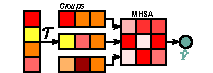
\includegraphics[width=\linewidth]{AttOmics_logo.pdf} }
         };
         \node[left=1cm of n4.west, anchor=east] (b4) {\tcbox[title=CrossAttOmics]{
                 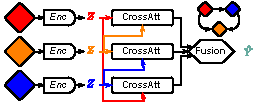
\includegraphics[width=\linewidth]{CrossAttOmics_Logo.pdf}}
         };
         \node[right=1cm of n5.east, anchor=west] (b5) {\tcbox[title=Counterfactuals]{TEST tesfkl fzlkfes gznjef fe,fbzkf vjnfzefb }};

         \draw[Prune, line width=1.5pt, -{Circle}] (n1.east) -- (b1.west);
         \draw[Prune, line width=1.5pt, -{Circle}] (n2.west) -- (b2.east);
         \draw[Prune, line width=1.5pt, -{Circle}] (n3.east) -- (b3.west);
         \draw[Prune, line width=1.5pt, -{Circle}] (n4.west) -- (b4.east);
         \draw[Prune, line width=1.5pt, -{Circle}] (n5.east) -- (b5.west);

         \tcbhypernode{\hyperref[chap:background]}{n1}
         \tcbhypernode{\hyperref[chap:sota]}{n2}
         \tcbhypernode{\hyperref[chap:attomics]}{n3}
         \tcbhypernode{\hyperref[chap:crossattomics]}{n4}
         \tcbhypernode{\hyperref[chap:counterfactuals]}{n5}

         \tcbhypernode{\hyperref[chap:background]}{b1}
         \tcbhypernode{\hyperref[chap:sota]}{b2}
         \tcbhypernode{\hyperref[chap:attomics]}{b3}
         \tcbhypernode{\hyperref[chap:crossattomics]}{b4}
         \tcbhypernode{\hyperref[chap:counterfactuals]}{b5}
     \end{tikzpicture}
 \end{center}

 %https://arxiv.org/abs/2206.00520
 %https://www.nature.com/articles/s41568-020-00327-9 % Designing deep learning studies in cancer diagnostics
\end{document}
